\begin{qu}[Coinciding orbits]\num
The circular orbits of satellites 1 and 2 coincide. Satellite 2 has
twice the mass of satellite 1. Compare their accelerations.

\vspace{20mm}

\includegraphics{mechanics/figs/gravity-coinciding-orbits}

A. 1's acceleration is half as much.

B. 1's acceleration is the same as 2's.

C. 1's acceleration is twice as much as 2's.

D. It depends on the periods of their orbits.
\end{qu}
